\begin{figure}
    \begin{subfigure}{.5\textwidth}
          \centering
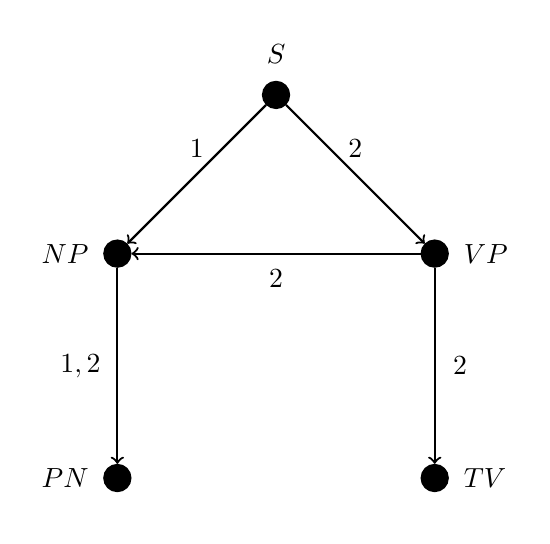
\begin{tikzpicture}[->,circle,draw,node distance=2.85cm,fill=black
                   ]

    \node[circle,label=90:$S$,draw,thick,fill=black](w0){$
    $};
    \node[circle,label=180:$NP$,below left of=w0,draw,thick,fill=black](w1){$
    $};
    \node[circle,label=0:$VP$,below right of=w0,draw,thick,fill=black](w2){$
    $};
    \node[circle,label=180:$PN$,below of=w1,draw,thick,fill=black](w3){$
    $};
    \node[circle,label=0:$TV$,below of=w2, draw,thick,fill=black](w4){$
    $};
    %\node[circle,label=90:$NP'$,below right of=w2, draw,thick,fill=black](w5){$
    %$};
    %\node[circle,label=0:$PN'$,below of=w5,draw,thick,fill=black](w6){$
    %$};
    \path[thick] (w0) edge [above] node {$1$} (w1)
    (w0) edge [above] node {$2$} (w2)
    (w1) edge [left] node {$1,2$} (w3)
    (w2) edge [right] node {$2$} (w4)
    (w2) edge [below] node {$2$} (w1);
    %(w5) edge [below] node {} (w6);

\end{tikzpicture} 
              \caption{Model for phase-structure}
                \label{example_linguistics}
    \end{subfigure}%
    \begin{subfigure}{.5\textwidth}
          \centering
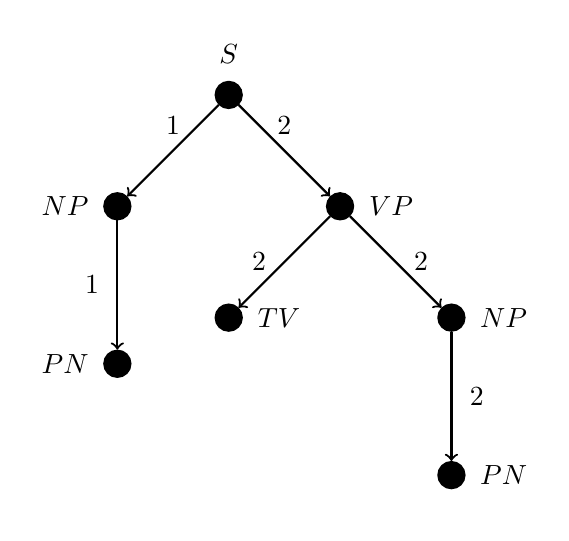
\begin{tikzpicture}[->,circle,draw,node distance=2cm,fill=black
                   ]

    \node[circle,label=90:$S$,draw,thick,fill=black](w0){$
    $};
    \node[circle,label=180:$NP$,below left of=w0,draw,thick,fill=black](w1){$
    $};
    \node[circle,label=0:$VP$,below right of=w0,draw,thick,fill=black](w2){$
    $};
    \node[circle,label=180:$PN$,below of=w1,draw,thick,fill=black](w3){$
    $};
    \node[circle,label=0:$TV$,below left of=w2, draw,thick,fill=black](w4){$
    $};
    \node[circle,label=0:$NP$,below right of=w2, draw,thick,fill=black](w5){$
    $};
    \node[circle,label=0:$PN$,below of=w5,draw,thick,fill=black](w6){$
    $};
    \path[thick] (w0) edge [above] node {$1$} (w1)
    (w0) edge [above] node {$2$} (w2)
    (w1) edge [left] node {$1$} (w3)
    (w2) edge [left] node {$2$} (w4)
    (w2) edge [right] node {$2$} (w5)
    (w5) edge [right] node {$2$} (w6);

\end{tikzpicture} 
              \caption{Tree-like model for phase-structure}
                \label{example_tree-like}
    \end{subfigure}
\end{figure}

